\documentclass[a4paper,11pt]{article}
\usepackage[utf8]{inputenc}
\usepackage[T1]{fontenc}
\usepackage[french]{babel}
\usepackage[right=2.3cm, left=2.3cm, bottom=3cm, top=2.2cm]{geometry}
\usepackage[ddmmyyyy]{datetime}
\usepackage[table]{xcolor}
\usepackage{lmodern,mathptmx,changepage,titlesec,hyperref,listings,lstautogobble,graphicx,array,longtable,multirow,lipsum,tikz,shorttoc,enumitem,float,verbatim, amsthm,amsfonts,amsmath,amssymb,mathrsfs,thmtools}
\usetikzlibrary{arrows,automata}
\usetikzlibrary{positioning}

\renewcommand{\rmdefault}{\sfdefault} %Utilisation de la police sans-serif ("Computer Modern Sans") pour la police roman
\renewcommand{\ttdefault}{pcr} 	%Utilisation d'une police "CourrierNew" pour la police monospaced (pour faire un listing manuel)
\linespread{1.15}				%Interligne

%Utilisation de liens colorés en bleu et soulignés
\hypersetup{colorlinks=true, urlcolor=blue, urlbordercolor=blue, linkcolor=black, linkbordercolor=white}
\makeatletter \Hy@AtBeginDocument{\def\@pdfborder{0 0 1} \def\@pdfborderstyle{/S/U/W 1}}\makeatother

\titlespacing*{\section} {0cm}{7ex plus 1ex minus .2ex}{1.5ex plus .2ex}
\titlespacing*{\subsection} {0cm}{4.5ex plus 1ex minus .2ex}{1.5ex plus .2ex}
\titleformat*{\section}{\huge\bfseries}
\titleformat*{\subsection}{\LARGE\bfseries}
\titleformat*{\subsubsection}{\normalsize\bfseries}

\definecolor{darkgreen}{rgb}{0,0.8,0}
\definecolor{mygray}{rgb}{0.93,0.93,0.93}
\definecolor{mymauve}{rgb}{0.58,0,0.82}
\lstset{	
	language=C,
	basicstyle=\small\ttfamily,
	backgroundcolor=\color{mygray},
	breaklines=true,
	breakatwhitespace=true,
	tabsize=3,
	captionpos=b,
	frame=none,
	rulecolor=\color{black},
	keywordstyle=\color{blue}\bfseries,
	stringstyle=\color{orange},
	showstringspaces=false,
	commentstyle=\footnotesize\color{darkgreen},
	keepspaces=true,
	extendedchars=true,
	numbers=left,
	numberstyle=\tiny\color{lightgray},
	stepnumber=1,
	escapeinside={(@}{@)},
	autogobble=true,
	literate=
		{á}{{\'a}}1 {é}{{\'e}}1 {í}{{}}1 {ó}{{\'o}}1 {ú}{{\'u}}1
		{Á}{{\'A}}1 {É}{{\'E}}1 {Í}{{\'I}}1 {Ó}{{\'O}}1 {Ú}{{\'U}}1
		{à}{{\`a}}1 {è}{{\`e}}1 {ì}{{\`i}}1 {ò}{{\`o}}1 {ù}{{\`u}}1
		{À}{{\`A}}1 {È}{{\'E}}1 {Ì}{{\`I}}1 {Ò}{{\`O}}1 {Ù}{{\`U}}1
		{ä}{{\"a}}1 {ë}{{\"e}}1 {ï}{{\"i}}1 {ö}{{\"o}}1 {ü}{{\"u}}1
		{Ä}{{\"A}}1 {Ë}{{\"E}}1 {Ï}{{\"I}}1 {Ö}{{\"O}}1 {Ü}{{\"U}}1
		{â}{{\^a}}1 {ê}{{\^e}}1 {î}{{\^i}}1 {ô}{{\^o}}1 {û}{{\^u}}1
		{Â}{{\^A}}1 {Ê}{{\^E}}1 {Î}{{\^I}}1 {Ô}{{\^O}}1 {Û}{{\^U}}1
		{œ}{{\oe}}1 {Œ}{{\OE}}1 {æ}{{\ae}}1 {Æ}{{\AE}}1 {ß}{{\ss}}1
		{ç}{{\c c}}1 {Ç}{{\c C}}1 {ø}{{\o}}1 {å}{{\r a}}1 {Å}{{\r A}}1
		{€}{{e}}1 {£}{{\pounds}}1 {«}{{\guillemotleft}}1
		{»}{{\guillemotright}}1 {ñ}{{\~n}}1 {Ñ}{{\~N}}1 {¿}{{?`}}1
}

%Redéfinition de la taille de \Huge pour le titre du document
\makeatletter\renewcommand\Huge{\@setfontsize\Huge{37pt}{40}}\makeatother
\date{\today}

\usepackage[french,frenchkw,ruled,vlined]{../texLib/algorithm2e}

\title{\vspace{\fill}\textbf{\Huge Rapport}}
\author{
	Frederick Coupvent Des Graviers - Sonny Klotz - Florian Lienhart - Thomas Momenzadeh
	\vspace{2em}\\
	\textit{Projet M1 Informatique}\\\textit{Accélération de Aitken quadratique}
	\vspace{2em}
}


\begin{document}
\pagenumbering{gobble}\clearpage
\maketitle\vspace{9em}
\begin{center}
\includegraphics[scale=0.7]{logo.png}\end{center}
\begin{flushright}Module \textit{Méthodes de ranking et recommandations}\end{flushright}

\newpage
\tableofcontents

\newpage\clearpage\pagenumbering{arabic}

	\section*{Introduction}
		\paragraph{}Le projet s'inscrit dans le cadre de l'UE \textbf{Méthodes de ranking et recommandations}, et plus particulièrement, nous étudierons l'algorithme \textit{Pagerank} de Google.
		\paragraph{}Cet algorithme a le rôle de classifier les pages web en attribuant une note de \textbf{pertinence} à chacune des pages. Pour entrer un peu plus dans détails, Google établit un graphe du web à l'aide des pages et des liens hypertextes contenues dans celle-ci.
		\paragraph{}La majeure problématique consiste à gérer efficacement la masse de données que représente le web. Ainsi, l'enjeu de \textit{Pagerank} va être de traiter efficacement en mémoire le calculer des notes de pertinence.
		\paragraph{}Ce document va présenter dans une première partie le choix de l'implémentation pour les structures de données utilisées. Nous allons ensuite parler de la méthode des puissances pour le calcul des pertinences pour ensuite étudier une variante, l'accélération de Aitken quadratique. Enfin, nous présenterons les résultats expérimentaux sur six graphes du web.
		
	\section{Structures de données}

	\subsection{Le graphe du web}
		
		\paragraph{}Les graphes du web sont représentées dans notre programme sous la forme d'une matrice du web. Chaque ligne de la matrice représente une page web et les valeurs non nulles indique qu'il existe un lien hypertexte vers une autre page.
		\paragraph{}La taille du web étant immense, les graphes pourront aussi être représentés par des fichiers de données volumineux. À titre d'exemple, le fichier \textit{wb-edu.txt} est un fichier d'une taille de 1 Go.
		\paragraph{}Il faut tout de même noter le caractère creux de notre matrice. En effet, la matrice de \textit{wb-edu.txt} contient environ $10^{7}$ lignes, ce qui nous donnerait, si on représente notre matrice entièrement, $10^{14}$ valeurs à stocker. Cependant cette matrice serait constituées majoritairement de zéros puisque l'on sait le nombre de valeurs non nulles à environ $6 \cdot 10^{7}$ valeurs ce qui est beaucoup plus envisageable en terme de mémoire.
		\paragraph{}L'enjeu va donc être d'implémenter les méthodes en exploitant au mieux le caractère creux de la matrice.
		
	\subsection{Implémentation}

		\paragraph{}Pour faire un choix d'implémentation convenable, il faut prendre de l'avance quant aux tâches réalisées par notre programme. L'essentiel de la complexité va reposer sur deux opérations, l'importation de la matrice à partir du fichier, et, le calcul des pertinences.
		\paragraph{}Le calcul des pertinences repose sur un produit vecteur-matrice. Soientt $n$ le nombre de noeuds du graphe du web, $\pi$ notre vecteur et $G$ notre matrice, le produit s'effectue de la manière suivante :
			\begin{align*}
				(\pi \cdot G)[i] = \sum_{j = 1}^{n} \pi[i] \cdot G[j, i]
			\end{align*}
		\paragraph{}On effectue $n$ produit vecteur-colonne. Ainsi pour pouvoir ignorer les valeurs nulles de $G$ (car elles ne modifient pas la valeur de la somme), il faut avoir un stockage de $G$ sur les \textbf{colonnes}.
		\paragraph{}Maintenant, pour ce qui est des fichiers utilisés, ils utilisent une structure organisée selon les lignes. Ainsi, notre travail va être de lire linéairement notre fichier pour stocker les arcs, puis d'effectuer un tri rapide pour réorganiser nos arcs en fonction des colonnes. Un tel travail s'effectue en $O(n \cdot log(n))$ en moyenne.

	\section{Méthode des puissances}
	Verif des resultats grace a scilab sur des graphes de petite taille, recup photos sur fcb thomas
	
	\subsection{Algorithme}
	\subsection{Principe}
	\subsection{Complexité}

	\section{Accélération de Aitken quadratique}

	\section{Résultats expérimentaux}
	
	\subsection{Description des données}
		\paragraph{}Pour étudier les performances des algorithmes, nous utilisons six graphes du web présentés dans le tableau ci-dessous :
		
			\begin{center}\begin{tabular}{clrrr}
				\hline
				Graphe du web & nb noeuds & nb arcs & taille \\
				\hline
				wb-cs-stanford & 9 914 & 36 854 & 624 Ko \\
				Stanford & 281 903 & 2 312 497 & 37 Mo \\
				Stanford-Berkeley & 683 446 & 7 583 376 & 120 Mo \\
				in-2004 & 1 382 908 & 16 917 053 & 277 Mo \\
				wikipedia & 1 634 989 & 19 753 078 & 309 Mo \\
				wb-edu & 9 845 725 & 57 156 537 & 1.06 Go \\
				\hline
			\end{tabular}\end{center}
		
		\paragraph{}À la consultation de ce tableau, il est forcé de constater du volume que représente ces données, ce qui justifie le choix des implémentations qui a été fait.
		\paragraph{}Nous voudrions signaler que suite au téléchargement du fichier \textit{Stanford-Berkeley} le nombre de lignes indiquées dans le fichier n'est pas correct, $68344$ au lieu de $683446$.
		\paragraph{}Le code source est en \textbf{langage C}, le contrôle de l'utilisation correcte de la mémoire a été effectué à l'aide de l'option \textbf{-g} du compilateur \textbf{gcc} et l'outil d'exécution \textbf{valgrind}. Cependant, l'utilisation de ces outils décuplent le temps de calcul, nous avons donc préparer une deuxième version sans debug pour l'utiliser arès avoir vérifier l'utilisation correcte de la mémoire.
		
	\subsection{Mesures de performances}
	
		\paragraph{}Nous vous présentons dans un premier temps les résultats en temps et en itérations de l'implémentation de la méthode des puissances et de l'accélération de aitken.
		
			\begin{center}\begin{tabular}{lrrrrrrr}
				\hline
				Graphe du web & nb noeuds & nb arcs & taille & Puis (ité) & Puis (sec) & Aitk (ité) & Aitk (sec) \\
				\hline
				wb-cs-stanford & 9 914 & 36 854 & 624 Ko & x & x & x & x \\
				Stanford & 281 903 & 2 312 497 & 37 Mo & x & x & x & x \\
				Stanford-Berkeley & 683 446 & 7 583 376 & 120 Mo & x & x & x & x \\
				in-2004 & 1 382 908 & 16 917 053 & 277 Mo & x & x & x & x \\
				wikipedia & 1 634 989 & 19 753 078 & 309 Mo & x & x & x & x \\
				wb-edu & 9 845 725 & 57 156 537 & 1.06 Go & x & x & x & x \\
				\hline
			\end{tabular}\end{center}
			
		\paragraph{}\colorbox{yellow}{commenter le tableau et décrire la machine utilisée RAM et Processeur}
		
		\paragraph{}Il est aussi intéressant d'avoir un compte-rendu visuel pour comparer les méthodes. Les graphes ci-dessous représentent la valeur de $log(\| \Pi^{(k + 1)} - \Pi^{(k)} \|_{1})$ en fonction de l'itération $k$ pour les deux méthodes implémentées pour les six graphes du web. Ces courbes ont été réalisées à l'aide du logiciel \textit{GNUPLOT}.
		\paragraph{}On rappelle les constantes utilisées : $\alpha = 0.85$ et $\epsilon = 10^{-6}$. Les courbes ont été ajustées à la même échelle pour pouvoir les comparer de manière visuelle.\\
		
		\begin{minipage}[c]{.46\linewidth}
			\begin{center}
				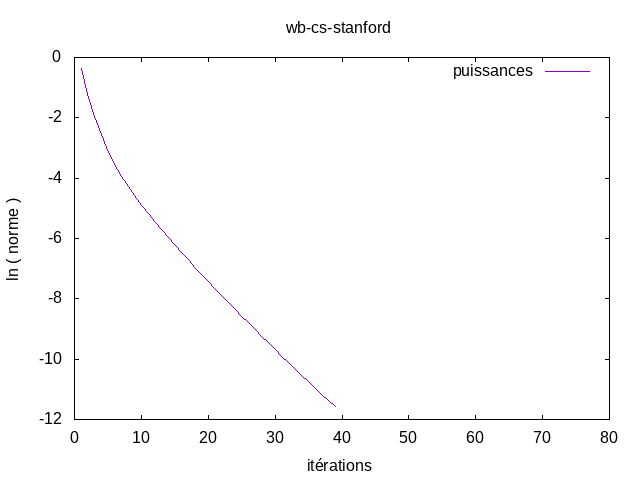
\includegraphics[scale=0.5]{plot-wb-cs-stanford.png}
			\end{center}
		\end{minipage} \hfill
		\begin{minipage}[c]{.46\linewidth}
			\begin{center}
				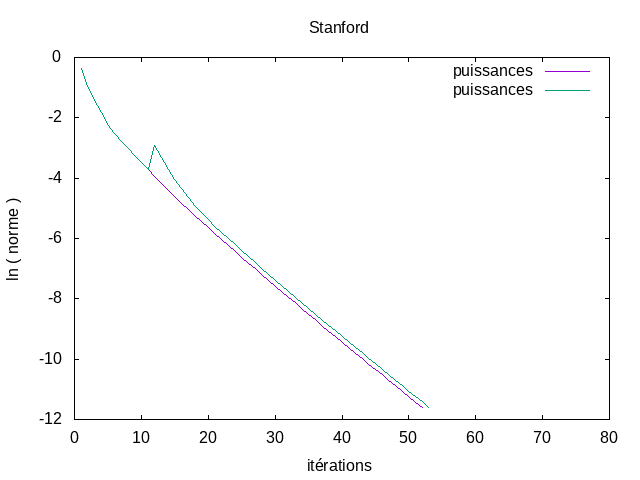
\includegraphics[scale=0.5]{plot-Stanford.png}
			\end{center}
		\end{minipage}
			

		
\end{document}
